\chapter{Week}
At the beginning of the week the first presentation 'Introduction to \ac{AI}' was held before the technical stuff of the company. The general background and principles of \ac{ML} have been introduced and an outlook given to the second presentation, which would go more into detail about the actual hardware realization. The rest of the week was spent going through various tutorials provided by Xilinx to familiarize myself with the workflow and the \ac{DNNDK} toolkit. As the state of tools used for \ac{AI} applications on \ac{FPGA} is still in flux, several approaches needed to be evaluated:
\begin{itemize}
	\item \textbf{\ac{DNNDK} workflow}: Version 2.08 of the toolkit supported only the Caffe neural network training framework and needs a network description file and the trained weights as input. The key component here is the \ac{DPU} \ac{IP} core provided by the \ac{DNNDK} toolkit. This core is integrated via Vivado into the block design of the hardware and can be configured and adjusted for several performance and power profiles.
	\item \textbf{\ac{DNNDK} \ac{SDSoC}}: Another option is to abstract away the whole Vivado block design process and use Xilinx \ac{SDSoC} to implement the whole system in a higher programming language, C++. Supported functions can then be flagged as being executed in the \ac{PL} part of the system. This approach makes using a traditional \ac{HDL} obsolete and is deemed more accessible. This approach uses the established Xilinx reVision stack for development providing high level \acp{API} for computer vision.
\end{itemize}
Furthermore, the \ac{IP} core provided by the \ac{DNNDK} toolkit was studied in more detail. A new base board was in the production state phase and the idea was to have a \ac{ML} design ready to showcase the capabilities of the new board.
\begin{figure}[!htb]
	\centering
		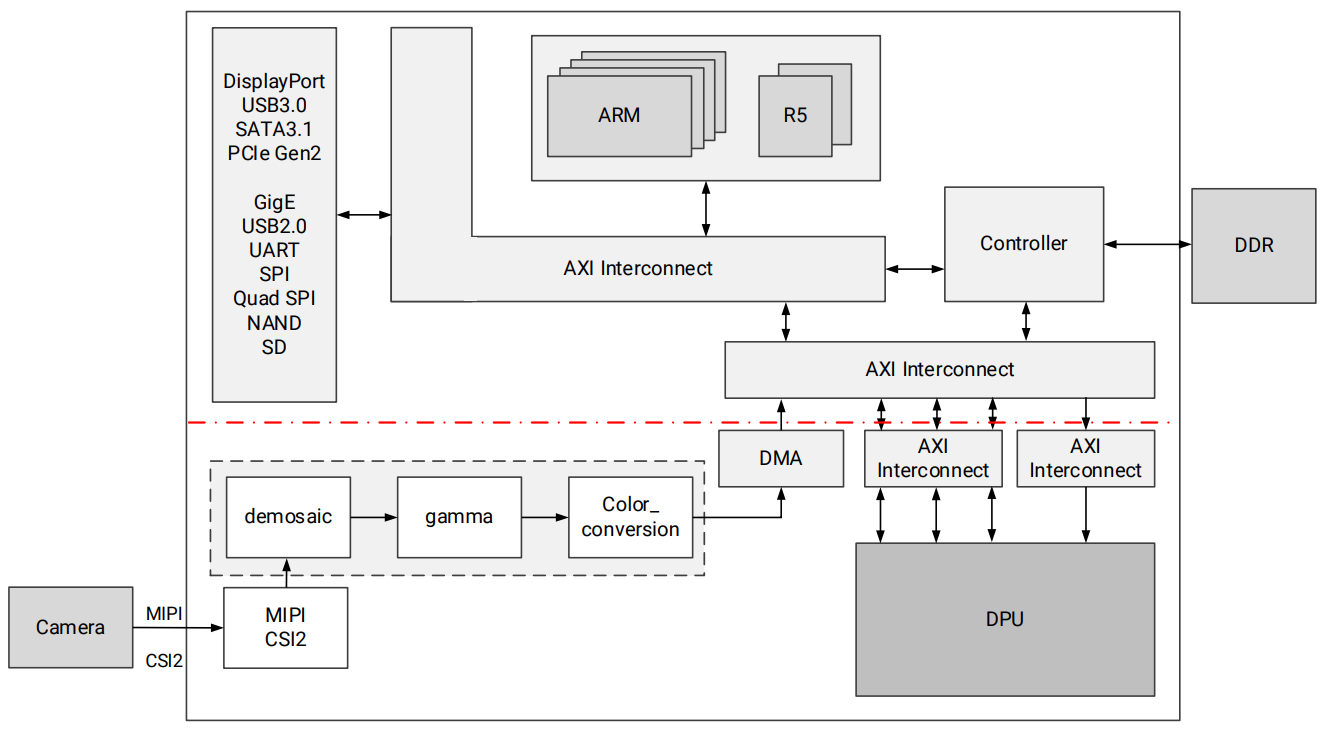
\includegraphics[width=\textwidth]{bilder/DPU_example_design.png}
		\caption{Example system with integrated \acs{DPU} \cite[p.~8]{dpu}}
		\label{fig:dpu_example}
\end{figure}
Figure~\ref{fig:dpu_example} shows an example hardware design with integrated \ac{DPU} module. In this example a camera is connected via the \ac{MIPI} \ac{CSI2} interface to the \ac{PS}. \ac{DMA} is usually used in conjunction with an \ac{AXI} interconnect to communicate with the \ac{PS}. The captured images are used as the input to the neural network and the \ac{DPU} itself can be viewed as a co-processor to the \ac{PS} implemented in the \ac{PL} fabric. The \ac{IP} core itself is customizable and the number of \ac{DPU} processor units, the size of the \ac{DPU} and the usage of \ac{DSP} blocks among other parameters are configurable. The decision on which size to use is based upon the performance demands of the application.